\documentclass[a4paper]{article}
\usepackage{fontspec}
\usepackage{fontenc}
\usepackage{extarrows}
\usepackage{chemfig}
\usepackage[version=4]{mhchem}
\usepackage{mwe}
\usepackage{amsmath}
\usepackage{fancyhdr}
\usepackage{color}
\usepackage{amssymb}
\usepackage{siunitx}
\usepackage{bigfoot}
\usepackage{fancyvrb}
\usepackage{tikz}
\usepackage{expl3}
\usepackage{calc}
\usepackage{geometry}
\geometry{left=2.5cm,right=2.5cm,top=2cm,bottom=3cm}
\usetikzlibrary{graphs, positioning, quotes, shapes.geometric}
\setmainfont{Hiragino Sans GB}

\title{元素化学笔记整理}
\author{胡译文}
\date{\today}

\pagestyle{fancy}
\fancyhead[L]{\footnotesize 化学笔记整理}
\fancyhead[R]{\footnotesize 胡译文}
\fancyfoot[C]{\thepage}

\makeatletter
\newcommand{\figcaption}{\def@captype{figure}\caption}
\newcommand{\tabcaption}{\def@captype{table}\caption}
\makeatother

\usepackage{hyperref}
\renewcommand\contentsname{目录}

\begin{document}
	\maketitle
	\begin{center}
		若有bug请到{\color{red}\href{https://github.com/huyiwen/Chem}{github}}上提Issue。
	\end{center}
	\renewcommand\contentsname{目录}
	\tableofcontents
	
	
	\clearpage
	\section*{Flashback}
	\subsection{金属活动顺序表}
	\begin{itemize}
		\item 钾钙钠镁铝:K Ca Na Mg Al
		\item 锌铁锡铅氢:Zn Fe Sn Pb H
		\item 铜汞银铂金:Cu Hg Ag Pt Au
	\end{itemize}
	
	
	\clearpage
	\section{\ce{Na}}
	\subsection{\ce{Na}单质}
	\subsubsection{物理性质}
	\begin{itemize}
		\item 银白色固体,有金属性光泽
		\item 密度介于水和煤油之间,用煤油或石蜡保存
		\item 熔点低
		\item 质地较软,可以用小刀切割
	\end{itemize}
	
	\subsubsection{化学性质}
		\paragraph{与非金属单质反应} 
			\begin{itemize}
				\item $\left\{\begin{array}{lr}
						\ce{4Na + O2 -> 2Na2O}\\
						\ce{2Na + O2 ->[\Delta] Na2O2}\\
					\end{array}\right.$
				\item $\ce{2Na + S -> Na2S}$
				\item $\ce{2Na + H2 ->[\Delta] 2NaH}$
				\item $\left\{\begin{array}{lr}
						\ce{2Na + Br2 -> 2NaBr}\\
						\ce{2Na + Cl2 ->[{点燃}] 2NaCl}\\
					\end{array}\right.$
			\end{itemize}
			\paragraph{与水反应}
			$\ce{2Na + 2H2O -> 2NaOH + H2 ^}$
			\begin{itemize}
				\item 浮:钠的密度比水小
				\item 溶:反应放热,钠的熔点低
				\item 游:生成氢气推动钠
				\item 响:反应剧烈
				\item 红:生成\ce{NaOH}遇到酚酞变红
			\end{itemize}
			\paragraph{与盐酸反应}
			$\ce{2Na + 2HCl -> 2NaCl + H2 ^}$
			\paragraph{与碱反应}
			实质是先与水反应,产物再和盐反应。
			\paragraph{与盐溶液反应}
			实质是先与水反应,产物再和盐反应(钠不能与盐溶液发生置换反应)。
			\begin{itemize}
				\item 钠与硫酸铜溶液
				$\left\{\begin{array}{lr}
					\ce{2Na + 2H2O -> 2NaOH + H2 ^}\\
					\ce{2NaOH + CuSO4 -> Na2SO4 + Cu(OH)2 v}\\
				\end{array}\right.$
			\end{itemize}
			\paragraph{与\ce{CO2}反应}
			$\left\{\begin{array}{lr}
				\ce{4Na + CO2 ->[\Delta] 2Na2O + C}\\
				\ce{4Na + 3CO2 ->[\Delta] 2Na2CO3 + C}\\
			\end{array}\right.$
		
	\subsubsection{钠的制取}
	$\left\{\begin{array}{lr}
		\ce{2NaCl(l) ->[{电解}] 2Na + Cl2 ^}\\
		\ce{2NaOH(l) ->[{电解}] 2Na + O2 ^ + H2 ^}\\
	\end{array}\right.$
	
	\subsubsection{钠的用途}
	\begin{itemize}
		\item 冶炼金属:$\ce{4Na + TiCl4(l) -> 4NaCl + Ti}$
		\item 原子反应导热剂
		\item 钠光灯
	\end{itemize}
	\subsubsection{焰色反应}
	\begin{itemize}
		\item 锂盐:\textcolor[rgb]{0.698,0.149,0.098}{深红色}
		\item 钠盐:\textcolor[rgb]{0.964,0.913,0.313}{黄色}
		\item 钾盐:\textcolor[rgb]{0.882,0.741,0.858}{紫色}(透过蓝色钴玻璃)
		\item 钙盐:\textcolor[rgb]{0.886,0.529,0.215}{砖红色}
		\item 锶盐:\textcolor[rgb]{0.698,0.152,0.107}{洋红色}
		\item 钡盐:\textcolor[rgb]{0.788,0.835,0.286}{黄绿色}
		\item 铜盐:\textcolor[rgb]{0.537,0.8,0.262}{绿色}
	\end{itemize}
	
	
	\subsection{\ce{Na}的化合物}
	
	\subsubsection{氧化钠和过氧化钠}
	\paragraph{比较氧化钠和过氧化钠}
	\renewcommand\arraystretch{2}
	\begin{center}
	\begin{tabular}{|c|c|c|}
		\hline
		名称&氧化钠&过氧化钠\\\hline
		化学式&\ce{Na2O}&\ce{Na2O2}\\\hline
		物理性质&白色固体&\textcolor[rgb]{0.968,0.898,0.686}{淡黄色}固体\\\hline
		氧化物类型&碱性氧化物&过氧化物\\\hline
		获取&$\ce{4Na + O2 -> 2Na2O}$&$\ce{2Na + O2 ->[\Delta] Na2O2}$\\\hline
		与水反应&$\ce{Na2O + H2O -> 2\underset{\text{白色粘稠物}}{\ce{NaOH}}}$&$\ce{2Na2O2 + 2H2O -> 4\underset{\text{白色粘稠物}}{\ce{NaOH}} + O2 ^}$\\\hline
		与酸反应&$\ce{Na2O + 2H+ -> 2Na+ + H2O}$&$\ce{2Na2O2 + 4H+ -> 4Na+ + 2H2O + O2 ^}$\\\hline
		与\ce{CO2}反应&$\ce{Na2O + CO2 -> Na2CO3}$&$\ce{2Na2O2 + 2CO2 -> 2Na2CO3 + O2}$\\\hline
		用途&制取烧碱&漂白剂、消毒剂、供氧剂\\\hline
	\end{tabular}
	\end{center}
	\paragraph{过氧化钠的强氧化性}
	\begin{itemize}
		\item 与\ce{SO2}反应:$\ce{Na2O2 + SO2 -> Na2SO4}$
		\item 投入\ce{FeCl2}溶液中生成\ce{Fe(OH)3}沉淀
		\item 投入氢硫酸,氧化硫化氢成硫单质,溶液浑浊
		\item 氧化\ce{SO3^2-}成\ce{SO4^2-}
		\item 使品红溶液褪色
	\end{itemize}
	
	\subsubsection{碳酸钠和碳酸氢钠}
	\paragraph{碳酸钠\ce{Na2CO3}}
	\begin{itemize}
		\item 俗名:纯碱、苏打
		\item 与盐酸反应:$\ce{Na2CO3 + 2HCl -> 2NaCl + H2O + CO2 ^}$
		\item 与\ce{Ca(OH)2}溶液反应:$\ce{Na2CO3 + Ca(OH)2 -> CaCO3 v + 2NaOH}$
		\item 与\ce{BaCl2}溶液反应:$\ce{Na2CO3 + BaCl2 -> BaCO3 v + 2NaCl}$
	\end{itemize}
	\paragraph{碳酸氢钠\ce{NaHCO3}}
	\begin{itemize}
		\item 俗名:小苏打
		\item 与盐酸反应:$\ce{NaHCO3 + HCl -> NaCl + H2O + CO2 ^}$
		\item 与过量\ce{Ca(OH)2}溶液反应:$\ce{Ca2+ + OH- + HCO3- -> CaCO3 v + H2O}$
		\item 与少量\ce{Ca(OH)2}溶液反应:$\ce{Ca2+ + 2OH- + 2HCO3- + Ca(OH)2 -> CaCO3 v + 2H2O + CO3^2-}$
		\item 与\ce{BaCl2}溶液反应:无明显现象
		\item 受热分解:$\ce{2NaHCO3 ->[\Delta] Na2CO3 + H2O + CO2 ^}$
	\end{itemize}
	\paragraph{相互转换}
	$\ce{Na2CO3 <=>[CO2 + H2O{或}H+][\Delta({固体}){或}OH-] NaHCO3}$
	\paragraph{鉴别\ce{Na2CO3}和\ce{NaHCO3}}
	\subparagraph{固体}
	根据热稳定性加热,能产生使澄清石灰水变浑浊的气体的是\ce{NaHCO3}
	\subparagraph{溶液}
	\begin{itemize}
		\item 与可溶性钙、钡盐生成沉淀的是\ce{Na2CO3}
		\item 与足量盐酸反应剧烈的是\ce{NaHCO3}
		\item 逐滴加盐酸先生成气体的是\ce{NaHCO3}
		\item 等物质的量pH值较大的是\ce{Na2CO3}
	\end{itemize}
	
	
	\clearpage
	\section{Mg和Al}
	\subsection{Mg单质和Al单质}
	\subsubsection{化学性质}
	\paragraph{与非金属单质反应}
	\begin{itemize}
		\item 与\ce{O2}反应:$\left\{\begin{array}{lr}
					\ce{2Mg + O2 ->[{点燃}] 2MgO}(耀眼白光)\\
					\ce{4Al + 3O2 ->[{点燃}] 2Al2O3}\\
				\end{array}\right.$
		\item 与\ce{CO2}反应:$\ce{2Mg + CO2 ->[{点燃}] 2MgO + C}(耀眼白光,黑色固体生成)$
		\item 与\ce{N2}反应:$\ce{3Mg + N2 ->[{点燃}] Mg3N2}$
		\item 与卤素反应:$\left\{\begin{array}{lr}
					\ce{2Mg + Cl2 ->[{点燃}] 2MgCl2}\\
					\ce{2Al + 3Cl2 ->[{点燃}] 2AlCl3}\\
				\end{array}\right.$
		\item 与硫反应:$\left\{\begin{array}{lr}
					\ce{Mg + S ->[\Delta] MgS}\\
					\ce{2Al + 3S ->[\Delta] Al2S3}\\
				\end{array}\right.$
	\end{itemize}
	注意,镁在空气中燃烧时会同时发生前三个反应。
	\paragraph{与热水反应}
	$\left\{\begin{array}{lr}
		\ce{Mg + H2O({沸水}) -> Mg(OH)2 + H2 ^}\\
		\ce{2Al + 6H2O -> 2Al(OH)3 + 3H2 ^}\\
	\end{array}\right.$
	\paragraph{与酸发生置换反应}
	特例:铝在冷的浓硫酸或浓硝酸中钝化。
	\paragraph{铝热反应}
	可以与\ce{FeO}、\ce{Fe2O3}、\ce{Fe3O4}、\ce{Cr2O3}、\ce{MnO2}、\ce{V2O5}等氧化物反应。\\
	$\left\{\begin{array}{lr}
		\ce{2Al + Fe2O3 ->[{高温}] Al2O3 + 2Fe}\\
		\ce{2Al + Cr2O3 ->[{高温}] Al2O3 + 2Cr}\\
	\end{array}\right.$
	\\用途:焊接金属、冶炼难溶金属。
	\paragraph{与碱反应}
	镁不与碱反应。铝与强碱发生反应:$\ce{2Al + 2NaOH + 6H2O -> 2NaAlO2 + 4H2O + 3H2 ^}$
	\subsubsection{制备}
	\paragraph{工业制铝}
	$\ce{2Al2O3(l) ->[{冰晶石}][{通电}] 4Al + 3O2 ^}$
	\paragraph{工业制镁}
	$\left\{\begin{array}{lr}
		\ce{Mg2+ + 2OH- -> Mg(OH)2 v}\\
		\ce{Mg(OH)2 + 2HCl -> MgCl2 + H2O}\\
		\ce{MgCl2(l) ->[{通电}] Mg + Cl2 ^}\\
	\end{array}\right.$
	\paragraph{海水提镁}
	$$
	\ce{\underset{\text{贝壳}}{CaCO3} -> CaO -> Ca(OH)2 -> Mg(OH)2 -> MgCl2 ->[{通电}] Mg}
	$$
	其中氯元素可以循环:$\ce{Cl2 -> HCl -> MgCl2 -> Cl2}$
	\paragraph{海水提溴}
	海水元素:溴
	$$
	\ce{{海水} ->[{晒盐}] {盐卤} ->[{通入}Cl2] Br2(aq) ->[{吹热空气或水蒸气}] Br2(g) ->[{热饱和纯碱}] {溴酸盐和溴盐溶液} ->[{稀硫酸酸化}] {Br2}}
	$$
	$\left\{\begin{array}{lr}
		\ce{Cl2 + 2Br- -> Br2 + 2Cl-}\\
		\ce{3Br2 + 3CO3^2- -> 5Br- + BrO3- + 3CO2}\\
		\ce{5Br- + BrO3- + 6H+ -> 3Br2 + 3H2O}\\
	\end{array}\right.$
	\paragraph{海带提碘}
	$$
	\ce{{海带} -> {烧碱灰} ->[{泡水浸取}] ->[Cl2] I2}
	$$
	
	
	\subsection{铝、氧化铝和氢氧化铝的两性}
	\paragraph{与酸反应}
	$\left\{\begin{array}{lr}
		\ce{2Al + 6H+ -> 2Al^3+ + 3H2 ^}({非氧化性酸})\\
		\ce{Al2O3 + 6H+ -> 2Al^3+ + 3H2O}\\
		\ce{Al(OH)3 + 3H+ -> Al^3+ + 3H2O}\\
	\end{array}\right.$
	\paragraph{与强碱反应}
	$\left\{\begin{array}{lr}
		\ce{2Al + 2OH- + 2H2O -> 2AlO2- + 3H2 ^}\\
		\ce{Al2O3 + 2OH- -> 2AlO2- + H2O}\\
		\ce{Al(OH)3 + OH- -> AlO2- + 2H2O}\\
	\end{array}\right.$
	\paragraph{\ce{Al(OH)3}的电离}
	$\left\{\begin{array}{lr}
		\ce{Al(OH)3 <=> H+ + AlO2- + H2O}\\
		\ce{Al(OH)3 <=> Al^3+ + OH-}\\
	\end{array}\right.$
	
	\subsection{铝离子和偏铝酸根}
	\subsubsection{铝离子}
	\paragraph{与\ce{NaOH}的相互滴加}
	缓慢滴加并搅拌
	\subparagraph{将\ce{NaOH}滴入\ce{Al^3+}溶液中}
	\begin{enumerate}
		\item 先出现白色沉淀:$\ce{Al^3+ + 3OH- -> Al(OH)3 v}\\$
		\item 后沉淀消失:$\ce{Al(OH)3 + OH- -> AlO2- + 2H2O}\\$
	\end{enumerate}
	\subparagraph{将\ce{Al^3+}滴入\ce{NaOH}溶液中}
	\begin{enumerate}
		\item 先无明显现象:$\ce{Al^3+ + 4OH- -> AlO2- + H2O}\\$
		\item 后产生白色沉淀:$\ce{Al^3+ + 3AlO2- + 6H2O -> 4Al3(OH)3 v}\\$
	\end{enumerate}
	\paragraph{与氨水反应}
	$\ce{Al^3+ + NH3*H2O -> Al(OH)3 v + 3NH4+}\\$
	\paragraph{双水解反应}
	\begin{itemize}
		\item $\ce{Al^3+ + 3HCO3- -> Al(OH)3 v + 3CO2 ^}$
		\item $\ce{Al^3+ + 3CO3^2- + 3H2O -> Al(OH)3 v + 3HCO3-}$
		\item $\ce{Al^3+ + 3AlO2- + 6H2O -> 4Al(OH)3 v}$
		\item $\ce{2Al^3+ + 3S^2- + 6H2O -> 2Al(OH)3 v + 3H2S ^}$
		\item $\ce{AlO2- + NH4+ + H2O -> 4Al(OH)3 v + NH3 ^}$
		\item $\ce{2Al^3+ + 3SiO3^2- + 6H2O -> 2Al(OH)3 v + 3H2SiO3 v}$
	\end{itemize}
	

	\subsubsection{偏铝酸根}
	\paragraph{与强酸相互滴加}缓慢滴加并搅拌
	\subparagraph{将\ce{H2SO4}滴入\ce{AlO2-}溶液中}
	\begin{enumerate}
		\item 先出现白色沉淀:$\ce{AlO2- + H+ + H2O -> Al(OH)3 v}\\$
		\item 后沉淀消失:$\ce{Al(OH)3 + 3H+ -> Al^3+ + 3H2O}\\$
	\end{enumerate}
	\subparagraph{将\ce{AlO2-}滴入\ce{H2SO4}溶液中}
	\begin{enumerate}
		\item 先无明显现象:$\ce{AlO2- + 4H+ -> Al^3+ + 2H2O}\\$
		\item 后产生白色沉淀:$\ce{Al^3+ + 3AlO2- + 6H2O -> 4Al3(OH)3 v}\\$
	\end{enumerate}
	\paragraph{与碳酸反应}
	立即生成\ce{Al(OH)3}沉淀且不溶解。
	\begin{itemize}
		\item \ce{CO2}过量:$\ce{AlO2- + 2H2O + CO2 -> Al(OH)3 v + HCO3-}\\$
		\item \ce{CO2}少量:$\ce{2AlO2- + 3H2O + CO2 -> 2Al(OH)3 v + CO3^2-}\\$
	\end{itemize}
	\paragraph{与铵盐溶液反应}
	$\ce{NH4+ + AlO2- + H2O -> Al(OH)3 v + NH3 ^}\\$
	
	\subsection{氢氧化铝}
	\subsubsection{物理性质}
	\begin{itemize}
		\item 白色胶状沉淀
	\end{itemize}
	\subsubsection{制备}
	\begin{itemize}
		\item $\ce{Al^3+ + NH3*H2O -> Al(OH)3 v + 3NH4+}\\$
		\item $\ce{AlO2- + 2H2O + CO2 -> Al(OH)3 v + HCO3-}\\$
		\item $\ce{Al^3+ + 3AlO2- + 6H2O -> 4Al3(OH)3 v}\\$
	\end{itemize}
	
	\subsection{总结}
	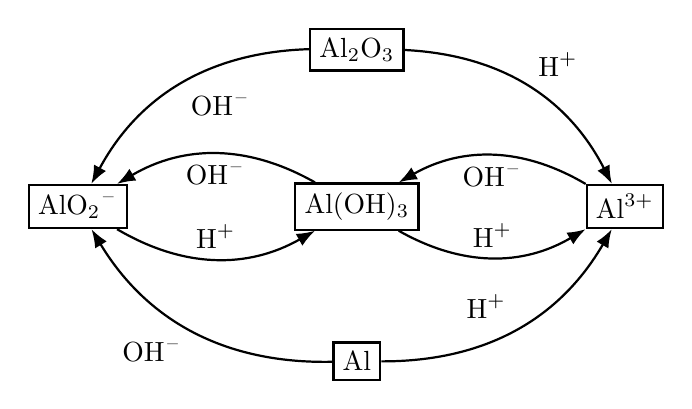
\begin{tikzpicture}[node distance=40pt, auto, thick]
		\node[draw] (Al2O3) {\ce{Al2O3}};
		\node[draw, below=of Al2O3] (AlOH) {\ce{Al(OH)3}};
		\node[draw, below=of AlOH] (Al) {\ce{Al}};
		\node[draw, right=60pt of AlOH] (Al3+) {\ce{Al^3+}};
		\node[draw, left=60pt of AlOH] (AlO2-) {\ce{AlO2-}};
		
		\draw[-Latex] (AlOH) [bend right] (AlO2-) edge node {\ce{H+}} (AlOH);
		\draw[-Latex] (AlO2-) [bend right] (AlOH) edge node {\ce{OH-}} (AlO2-);
		\draw[-Latex] (Al3+) [bend right] (AlOH) edge node {\ce{H+}} (Al3+);
		\draw[-Latex] (AlOH) [bend right] (Al3+) edge node {\ce{OH-}} (AlOH);
		\draw[-Latex] (Al3+) [bend left] (Al2O3) edge node {\ce{H+}} (Al3+);
		\draw[-Latex] (AlO2-) [bend right] (Al2O3) edge node {\ce{OH-}} (AlO2-);
		\draw[-Latex] (Al3+) [bend right] (Al) edge node {\ce{H+}} (Al3+);
		\draw[-Latex] (AlO2-) [bend left] (Al) edge node {\ce{OH-}} (AlO2-);
	\end{tikzpicture}
	
	
	\clearpage
	\section{Fe}
	\subsection{铁单质}
	\subsubsection{物理性质}
	\begin{itemize}
		\item 银白色固体,有金属性光泽;
		\item 容易被磁铁吸引;
		\item 地壳中居第四位;
	\end{itemize}
	
	\subsubsection{化学性质}
		铁元素性质活泼,有较强的还原性,主要化合价为+2价和+3价。
		\paragraph{与非金属单质反应} 
			\begin{itemize}
				\item $\ce{3Fe + 2O2 ->[{点燃}] Fe3O4}$
				\item $\ce{2Fe + 3Cl2 ->[{点燃}] FeCl3}$
				\item $\ce{Fe + S ->[\Delta] FeS}$
			\end{itemize}
		\paragraph{与水反应}
		铁在高温下与水蒸气反应
		$\ce{3Fe + 4H2O(g) ->[{高温}] Fe3O4 + 4H2}$
		\paragraph{与酸反应}
		铁遇到冷的浓硫酸或浓硝酸会钝化。
		\begin{itemize}
			\item 与非还原性酸:$\ce{Fe + 2H+ -> Fe^2+ + H2 ^}$
			\item 与还原性酸:$\ce{Fe + 4H+ + NO3- -> Fe^3+ + NO ^ + 2H2O}$
		\end{itemize}
		\paragraph{与盐溶液反应}
			\begin{itemize}
				\item 置换反应:$\ce{Fe + Cu^2+ -> Fe^2+ + Cu}$
				\item 与氯化铁溶液:$\ce{Fe + 2Fe^3+ -> 3Fe^2+}$ 
			\end{itemize}
			
	\subsection{铁的氧化物}
	\renewcommand\arraystretch{2}
	\begin{center}
	\begin{tabular}{|c|p{0.3\textwidth}<{\centering}|p{0.3\textwidth}<{\centering}|p{0.3\textwidth}<{\centering}|}
		\hline
		名称&氧化亚铁&氧化铁&四氧化三铁\\\hline
		俗称&-&铁红&磁性氧化铁\\\hline
		化学式&\ce{FeO}&\ce{Fe2O3}&\ce{Fe3O4}\\\hline
		化合价&+2&+3&+2、+3\\\hline
		物理性质&黑色粉末&\textcolor[rgb]{0.541,0.149,0.078}{红褐色}粉末&黑色晶体\\\hline
		与\ce{CO}反应&$\ce{FeO + CO ->[\Delta] Fe + CO2}$&$\ce{Fe2O3 + 3CO ->[\Delta] 2Fe + 3CO2}$&$\ce{Fe3O4 + 4CO ->[\Delta] 3Fe + 4CO2}$\\\hline
		与\ce{H2}反应&$\ce{FeO + H2 ->[\Delta] Fe + H2O}$&$\ce{Fe2O3 + 3H2 ->[\Delta] 2Fe + 3H2O}$&$\ce{Fe3O4 + 4H2 ->[\Delta] 3Fe + 4H2O}$\\\hline
		与酸反应&$\ce{FeO + 2H+ -> Fe^2+ + H2O}$&$\ce{Fe2O3 + 6H+ -> 2Fe^3+ + 3H2O}$&$\ce{Fe3O4 + 8H+ -> Fe^2+ + 2Fe^3+ + 4H2O}$\\\hline
	\end{tabular}
	\end{center}

	\subsection{铁的水化物}
	\subsubsection{比较\ce{Fe(OH)2}和\ce{Fe(OH)3}}
	\begin{center}
	\begin{tabular}{|c|c|c|}
		\hline
		名称&氢氧化亚铁&氢氧化铁\\\hline
		化学式&\ce{Fe(OH)2}&\ce{Fe(OH)3}\\\hline
		物理性质&白色固体&\textcolor[rgb]{0.541,0.149,0.078}{红褐色}固体\\\hline
		与酸反应&$\ce{Fe(OH)2 + 2H+ -> Fe^2+ + 2H2O}$&$\ce{Fe(OH)3 + 3H+ -> Fe^3+ + 3H2O}$\\\hline
		受热分解&$\ce{Fe(OH)2 ->[\Delta] FeO + H2O}$&$\ce{2Fe(OH)3 ->[\Delta] Fe2O3 + 3H2O}$\\\hline
		制备&$\ce{FeCl2 + 2NaOH -> Fe(OH)2 v + 2NaCl}$&$\ce{FeCl3 + 3NaOH -> Fe(OH)3 v + 3NaCl}$\\\hline
	\end{tabular}
	\end{center}
	\subsubsection{\ce{Fe(OH)2}和\ce{Fe(OH)3}的转化}
	\ce{Fe(OH)2}在空气中可以迅速被氧化成\ce{Fe(OH)3}。现象是由\textbf{白色絮状沉淀}迅速变成\textcolor[rgb]{0.231,0.301,0.219}{灰绿色},最后变成\textcolor[rgb]{0.541,0.149,0.078}{红褐色}。
	反应方程式:\ce{4Fe(OH)2 + O2 + 2H2O -> 4Fe(OH)3}。
	
	\subsection{铁三角(铁、亚铁盐、铁盐)}
	\begin{tikzpicture}[node distance=40pt, auto, thick]
		\node[draw] (Fe) {\ce{Fe}};
		\node[below=104pt of Fe] (TEMP) {};
		\node[draw, right=60pt of TEMP] (Fe3+) {\ce{Fe^3+}};
		\node[draw, left=60pt of TEMP] (Fe2+) {\ce{Fe^2+}};
		
		\draw[-Latex] (Fe) (Fe3+) edge node {\ce{Cl2}} (Fe);
		\draw[-Latex] (Fe3+) [bend left] (Fe) edge node {\ce{Zn}} (Fe3+);
		\draw[-Latex] (Fe3+) (Fe2+) edge node {\ce{Fe}或\ce{Cu}} (Fe3+);
		\draw[-Latex] (Fe2+) [bend left] (Fe3+) edge node {\ce{HNO3}或\ce{Cl2}} (Fe2+);
		\draw[-Latex] (Fe2+) (Fe) edge node {\ce{Zn}} (Fe2+);
		\draw[-Latex] (Fe) [bend left] (Fe2+) edge node {\ce{Fe^3+}或\ce{H+}} (Fe);
	\end{tikzpicture}
	\paragraph{亚铁盐}
	含有\ce{Fe^2+}的溶液呈\textcolor[rgb]{0.625,0.8,0.7}{浅绿色},\ce{Fe^2+}既有氧化性,又有还原性。
	\paragraph{铁盐}
	含有\ce{Fe^3+}的溶液呈\textcolor[rgb]{0.835,0.611,0.247}{棕黄色}, \ce{Fe^3+}具有氧化性。含有\ce{Fe^3+}的盐溶液遇到\ce{KSCN}溶液时变成红色。
	
	
	\clearpage
	\section{Si}
	\subsection{硅单质}
	\subsubsection{物理性质}
	\begin{itemize}
		\item 分类:无定形硅、晶体硅(结构类似金刚石)
		\item 灰黑色晶状固体
		\item 质地较脆
		\item 半导体
	\end{itemize}
	\subsubsection{化学性质}
	\paragraph{与非金属单质反应} 
		\begin{itemize}
			\item $\ce{Si + O2 ->[{高温}] SiO2}$
			\item $\ce{Si + 2Cl2 ->[\Delta] SiCl4}$
			\item $\ce{Si + 2F2 -> SiF4}$
			\item $\ce{Si + C ->[{高温}] \underset{\text{金刚砂}}{SiC}}$
		\end{itemize}
	\paragraph{与水反应}
	$\underbrace{\ce{Si + H2O + 2NaOH -> Na2SiO3 + 2H2 ^}}_{\text{野外制氢}}$
		
	\subsection{硅的氧化物}
	\subsubsection{物理性质}
	\begin{itemize}
		\item 透明、硬度大、熔点高
	\end{itemize}
	\subsubsection{化学性质}
	\paragraph{酸性氧化物}
	\subparagraph{与强碱反应}
	$\underbrace{\ce{SiO2 + 2NaOH -> Na2SiO3 + H2O}}_{\text{装NaOH溶液不用玻璃塞}}$
	\subparagraph{与唯一一种酸氢氟酸反应}
	$\underbrace{\ce{SiO2 + 4Hf -> SiF2 ^ + 2 H2O}}_{\text{腐蚀玻璃、玻璃雕花}}$
	\subparagraph{与碱性氧化物反应}
	氧化硅与碱性氧化物反应,不与水反应(与水反应产物为硅酸,是沉淀,阻止反应进行)
	\begin{itemize}
		\item $\ce{SiO2 + Na2O ->[{高温}] Na2SiO3}$
		\item $\ce{SiO2 + CaO ->[{高温}] CaSiO3}$
	\end{itemize}
	\subparagraph{与碱性盐反应}
	\begin{itemize}
		\item $\underbrace{\ce{SiO2 + Na2CO3 ->[{高温}] Na2SiO3 + CO2 ^}}_{\text{制作玻璃}}$
		\item $\underbrace{\ce{SiO2 + CaCO3 ->[{高温}] CaSiO3 + CO2 ^}}_{\text{造渣反应}}$
	\end{itemize}
	\subparagraph{与碳反应}
	\begin{itemize}
		\item $\ce{SiO2 + 2C ->[{高温}] Si + 2CO ^}$
		\item $\ce{SiO2 + 3C ->[{高温}] SiC + 3CO ^}$
	\end{itemize}
	\subparagraph{精炼}
	\begin{enumerate}
		\item $\ce{SiO2 + 4Mg ->[{高温}] Mg2Si + 2MgO}$
		\item $\ce{Mg2Si + 4HCl -> 2MgCl2 + SiH4 ^}$
		\item $\ce{SiH4 + 2O2 -> SiO2 + 2H2O}$(自然)
	\end{enumerate}

	
	\subsection{硅的水化物(硅酸、原硅酸)}
	硅酸:\ce{H2SiO3}、、
	原硅酸:\ce{H4SiO4}
	\subsubsection{物理性质}
	白色胶状沉淀
	\subsubsection{化学性质}
	\paragraph{弱酸性}
	不使酸碱指示剂变色
	\subparagraph{硅酸电离}
	$\left\{\begin{array}{lr}
		\ce{H2SiO3 <=> H+ + HSiO3-}\\
		\ce{H2SiO3- <=> H+ + SiO3^2-}\\
	\end{array}\right.$
	\subparagraph{原硅酸电离}
	$\left\{\begin{array}{lr}
		\ce{H4SiO4 <=> H+ + H3SiO4-}\\
		\ce{H3SiO4- <=> H+ + H2SiO4^2-}\\
		\ce{H2SiO4- <=> H+ + HSiO4^3-}\\
		\ce{HSiO4- <=> H+ + SiO4^4-}\\
	\end{array}\right.$
	\paragraph{不稳定沉淀}
	\begin{itemize}
		\item $\ce{H4SiO4 -> H2SiO3 + H2 ^}$
		\item $\ce{H2SiO3 ->[\Delta] SiO2 + H2O}$
		\item $\ce{H2SiO3 ->[\Delta] SiO2*xH2O + H2O}$
	\end{itemize}
	\paragraph{与强碱反应}
	\subparagraph{与氢氧化钠反应}
	$\ce{H2SiO3 + 2NaOH -> Na2SiO3 + 2H2O}$
	\subparagraph{不与氨气反应}
	$\ce{SiO3^2- + 2NH4+ -> H2SiO3 v + 2NH3 ^}$
	\subsubsection{制备}
	\paragraph{\ce{SiO2}无法一步变成\ce{H2SiO3}}
	$\left\{\begin{array}{lr}
		\ce{SiO2 + 2NaOH -> Na2SiO3 + H2O}\\
		\ce{Na2SiO3 + 2HCl -> 2NaCl + H2SiO3 v}\\
	\end{array}\right.$
	
	\subsection{硅酸盐}
	\subsubsection{物理性质}
	\ce{K2SiO3}和\ce{Na2SiO3}溶于水,其余硅酸盐微溶于水。
	\subsubsection{化学性质}
	\begin{itemize}
		\item $\left\{\begin{array}{lr}
					\ce{Na2SiO3 + CO2 + H2O -> Na2CO3 + H2SiO3 v}\\
					\ce{Na2SiO3 + 2CO2 + 2H2O -> 2NaHCO3 + H2SiO3 v}\\
				\end{array}\right.$
		\item $\left\{\begin{array}{lr}
					\ce{Na2SiO3 + 6HF -> SiF4 ^ + 2NaF + 3H2O}\\
					\underbrace{\ce{CaSiO3 + 6HF -> SiF4 ^ + CaF2 + 3H2O}}_{\text{产物硅酸不稳定生成\ce{SiO2},继续与氢氟酸反应}}\\
				\end{array}\right.$
	\end{itemize}
	\subsubsection{硅酸盐的拆分}
	$活泼金属氧化物\longrightarrow 较活泼金属氧化物\longrightarrow 二氧化硅\longrightarrow 水$
	\begin{itemize}
		\item \ce{Na2SiO3}:\ce{Na2O*SiO2}
		\item \ce{CaSiO3}:\ce{CaO*SiO2}
		\item \ce{Al2(Si2O5)(OH)4)}:\ce{Al2O3*2SiO2*2H2O}
	\end{itemize}
	
	\subsection{用途与俗称}
	\subsubsection{用途}
	\begin{itemize}
		\item \ce{Si}(不透明):硅芯片、太阳能电池板
		\item \ce{SiO2}(透明):玻璃、石英玻璃、硅胶(\ce{mSiO2*nH2O},干燥剂)、光导纤维
		\item \ce{SiO3^2-}盐:水泥、陶瓷、防火材料等无机非金属材料
		\item \ce{H2SiO3}:制硅胶
	\end{itemize}
	\subsubsection{俗称}
	\begin{itemize}
		\item \ce{SiO2}:水晶、玛瑙、石英
		\item \ce{Na2SiO3}水溶液:水玻璃
		\item \ce{Na2SiO3}:泡花碱
	\end{itemize}
	
	
	\clearpage
	\section{Cl}
	\paragraph{氯相关}
	\subparagraph{含氯酸}
	从上至下,酸性递增,氧化性递减。
	\begin{itemize}
		\item \ce{HClO}:次氯酸
		\item \ce{HClO2}:亚氯酸
		\item \ce{HClO3}:氯酸
		\item \ce{HClO4}:高氯酸
	\end{itemize}
	\subparagraph{卤素}
	\ce{F}、\ce{Cl}、\ce{Br}、\ce{I}
	\subparagraph{拟卤素}
	$\underset{\text{氰}}{\ce{CN}}$、$\underset{\text{硫氰}}{\ce{SCN}}$、$\underset{\text{氧氰}}{\ce{OCN}}$
	
	\subsection{盐酸}
	\subsubsection{物理性质}
	无色、有刺激性气味液体。
	\subsubsection{化学性质}
	\paragraph{酸性}
	产物中有盐
	\begin{itemize}
		\item $\ce{2H+ + Fe -> Fe^2+ + H2 ^}$
		\item $\ce{H+ + OH- -> H2O}$
		\item $\ce{2H+ + CaO -> Ca2+ + H2O}$
		\item $\ce{2H+ + CO3^2- -> CO2 ^ + H2O}$
	\end{itemize}
	\paragraph{氧化性}
	盐酸的氧化性由\ce{H+}体现
	\begin{itemize}
		\item $\ce{2H+ + Fe -> Fe^2+ + H2 ^}$
	\end{itemize}
	\paragraph{还原性}
	\begin{itemize}
		\item $\underbrace{\ce{4HCl({浓}) + MnO2 ->[\Delta] MnCl2 + CL2 ^ + 2H2O}}_{\text{实验室制氯气}}$
		\item $\left\{\begin{array}{lr}
				\ce{16HCl + 2KMnO4 -> 2KCl + 5Cl2 ^ + 2MnCl2 + 8H2O}\\
				\ce{14HCl + K2Cr2O7 -> 2KCl + 3Cl2 ^ + 2CrCl3 + 7H2O}\\
				\ce{6HCl + KClO3 -> KCl + 3Cl2 ^ + 3H2O}\\
				\ce{14HCl + PbO2 -> PbCl2 + Cl2 ^ + 2H2O}\\
				\ce{6HCl + NaBiO3 -> NaCl + Cl2 ^ + BiCl2 + 3H2O}\\
			\end{array}\right.$
	\end{itemize}
	\subsubsection{制备}
	\paragraph{工业}
	\begin{enumerate}
		\item $\ce{2NaCl + 2H2O ->[{通电}] 2NaOH + H2 ^ + Cl2 ^}$
		\item $\ce{H2 + Cl2 ->[{点燃}] 2HCl}$
	\end{enumerate}
	\paragraph{实验室}
	\begin{itemize}
		\item $\ce{NaCl + H2SO4({浓}) ->[\Delta] NaHSO4 + HCl ^}$
		\item $\ce{2NaCl + H2SO4({浓}) ->[\Delta] Na2SO4 + 2HCl ^}$
	\end{itemize}
	\subsection{氯气}
	\subsubsection{物理性质}
	\begin{itemize}
		\item \textcolor[rgb]{0.745,0.752,0.317}{黄绿色}气体
		\item 密度大于空气,加压易液化
		\item 难溶于饱和食盐水,可溶于水,易溶于\ce{CCl4}。
	\end{itemize}
	\subsubsection{化学性质}
	\paragraph{助燃性}
	强氧化性
	\begin{itemize}
		\item $\ce{H2 + Cl2 ->[{点燃}] 2HCl}$(苍白色火焰)
		\item $\ce{2Fe + 3Cl2 ->[{点燃}] 2FeCl3}$(产物是三价铁)
		\item $\ce{Cu + Cl2 ->[{点燃}] CuCl2}$
		\item $\ce{2Na + Cl2 ->[{点燃}] 2NaCl}({白烟黄光})$
		\item 磷在氯气中燃烧产生白色烟雾$\left\{\begin{array}{lr}
				\ce{2P + 5Cl2 ->[{点燃}] 2PCl5}({烟})\\
				\ce{2P + 3Cl2 ->[{点燃}] 2PCl3}({雾})\\
			\end{array}\right.$
		\item $\left\{\begin{array}{lr}
				\ce{PCl3 + 3H2O -> H3PO3 + 3HCl}\\
				\ce{PCl5 + 4H2O -> H3PO4 + 5HCl}\\
			\end{array}\right.$
	\end{itemize}
	\paragraph{氧化性和还原性}
	\begin{itemize}
		\item $\left\{\begin{array}{lr}
				\ce{H2O + Cl2 <=> HCl + HClO}\\
				\ce{H2O + Cl2 <=> H+ + Cl- + HClO}\\
			\end{array}\right.$
		\item $\left\{\begin{array}{lr}
				\ce{NaOH + Cl2 -> NaCl + \underset{\text{84消毒液、漂白粉}}{NaClO} + H2O}\\
				\ce{2Ca(OH)2 + 2Cl2 -> CaCl2 + \underset{\text{漂白精、漂白粉}}{Ca(ClO)2} + 2H2O}\\
			\end{array}\right.$
		\item $\left\{\begin{array}{lr}
				\ce{6NaOH + 3Cl2 ->[\Delta] 5NaCl + NaClO3 + 3H2O}\\
				\ce{6KOH + 3Cl2 ->[\Delta] 5KCl + KClO3 + 3H2O}\\
			\end{array}\right.$
		\item $\ce{2H2O + Cl2 + SO2 -> HCl + H2SO4}$
	\end{itemize}
	\subsubsection{制备}
	\paragraph{工业}
	\begin{itemize}
		\item $\ce{2NaCl + 2H2O ->[{通电}] 2NaOH + H2 ^ + Cl2 ^}$
		\item $\ce{2NaCl(l) ->[{通电}] 2Na + Cl2 ^}$
	\end{itemize}
	\paragraph{实验室}
	\begin{itemize}
		\item $\ce{MnO2 + 4HCl({浓}) ->[\Delta] Cl2 ^ + MnCl2 + 2H2O}$
	\end{itemize}
	\subsubsection{除杂}
	\begin{itemize}
		\item \ce{Cl2}(\ce{HCl}):饱和食盐水(溶液度:\ce{HCl} > \ce{NaCl} > \ce{Cl2})
		\item \ce{HCl}(\ce{Cl2}):\ce{CCl4}
		\item \ce{CO2}(\ce{HCl}):饱和\ce{NaHCO3}溶液
	\end{itemize}
	\subsubsection{氯水}
	\paragraph{成分}
	\begin{itemize}
		\item 分子:\ce{H2O}、\ce{Cl2}、\ce{HClO}
		\item 离子:\ce{Cl-}、\ce{H+}、\ce{ClO-}、\ce{OH-}
	\end{itemize}
	\paragraph{检验}
	\begin{itemize}
		\item \ce{Cl2}:\ce{FeCl2}溶液由\textcolor[rgb]{0.625,0.8,0.7}{浅绿色}变为\textcolor[rgb]{0.835,0.611,0.247}{棕黄色}
		\item \ce{Cl-}:加入硝酸酸化的\ce{AgNO3}溶液,产生白色沉淀
		\item \ce{HClO}:有色布条褪色
		\item \ce{H+}:pH试纸先变红,再褪色
	\end{itemize}
	\subsubsection{鉴别}
	湿润淀粉碘化钾试纸变为\textcolor[rgb]{0.556,0.827,0.898}{蓝色}
	$\ce{Cl2 + 2KI -> 2KCl + I2}$
	\subsection{次氯酸}
	\paragraph{化学式}
	\ce{HClO}
	\subsubsection{化学性质}
	\paragraph{见光分解}
	$\ce{2HClO ->[{光}] 2HCl + O2 ^}$
	\paragraph{酸性}
	\ce{H2CO3} > \ce{HClO} > \ce{HCO3-}
	\paragraph{氧化性}
	$\ce{HClO + SO2 + H2O -> HCl + H2SO4}$
	\subsection{含氯酸盐}
	\subsubsection{\ce{NaClO}}
	\paragraph{次氯酸钠的变质}
	$\left\{\begin{array}{lr}
		\ce{CO2 + NaClO + H2O -> HClO + NaHCO3}\\
		\ce{2HClO ->[{光}] 2HCl + O2 ^}\\
	\end{array}\right.$
	\paragraph{\ce{SO2}通入\ce{NaClO3}溶液}
	$\ce{ClO- + SO2 + H2O -> Cl- + 2H+ + SO4^2-}$
	\subsubsection{\ce{Ca(ClO)2}}
	\paragraph{次氯酸钙的变质}
	$\left\{\begin{array}{lr}
		\ce{CO2 + Ca(ClO)2 + H2O -> 2HClO + CaCO3 v}\\
		\ce{2HClO ->[{光}] 2HCl + O2 ^}\\
	\end{array}\right.$
	\paragraph{\ce{SO2}通入\ce{Ca(ClO3)2}溶液}
	$\ce{Ca^2+ + ClO- + SO2 + H2O -> Cl- + 2H+ + CaSO4 v}$
	\subsubsection{\ce{Cl2}逐渐通入\ce{FeI2}和\ce{FeBr2}混合溶液}
	\begin{enumerate}
		\item $\ce{Cl2 + 2I- -> 2Cl- + I2}$
		\item $\ce{Cl2 + 2Fe^2+ -> 2Cl- + 2Fe^3+}$
		\item $\ce{Cl2 + 2Br- -> 2Cl- + Br2 ^}$
		\item $\ce{5Cl2 + 6H2O + I2 -> 12H+ + 2IO3- + 10Cl-}$
	\end{enumerate}
	\subsubsection{\ce{Cl2}逐渐通入\ce{Na2CO}溶液}
	\begin{equation}\label{equ:E1}
			\ce{H2O + Cl2 <=> HCl + HClO}
	\end{equation}
	\begin{equation}\label{equ:E2}
			\ce{HCl + Na2CO3 -> NaCl + NaHCO3}
	\end{equation}
	\begin{equation}\label{equ:E3}
			\ce{HCl + NaHCO3 -> NaCl + H2O + CO2 ^}
	\end{equation}
	\begin{equation}\label{equ:E4}
			\ce{HClO + Na2Co3 <=> NaClO + NaHCO3}
	\end{equation}
	注意\ce{HClO}和\ce{NaHCO3}不反应。
	\begin{enumerate}
		\item $\ce{2Na2CO3 + Cl + H2O -> 2NaHCO3 + NaCl + NaClO}$(\ref{equ:E1}+\ref{equ:E2}+\ref{equ:E4})
		\item $\ce{Cl2 + Na2CO3 + H2O -> NaCl + NaHCO3 + HClO}$(\ref{equ:E1}+\ref{equ:E2})
		\item $\ce{Na2CO3 + 2Cl2 + H2O -> CO2 ^ + 2NaCl + 2HClO}$(\ref{equ:E1}+\ref{equ:E2}+\ref{equ:E3})
	\end{enumerate}
	
	
	
	\clearpage
	\section{S}
	
	\subsection{硫化氢}
	\subsubsection{物理性质}
	\begin{itemize}
		\item 无色、有刺激性气味(臭鸡蛋味)、有毒气体
		\item 能溶于水
		\item \ce{H2S}水溶液俗称氢硫酸,有毒
		\begin{itemize}
		\item 碘酸:\ce{HIO}
		\item 碘化氢:\ce{HI}
		\item 氢碘酸:\ce{HI}水溶液
		\end{itemize}
	\end{itemize}
	\subsubsection{化学性质}
	\paragraph{弱酸性}
	\subparagraph{与碱生成对应酸式/正盐}
	\subparagraph{与一些盐反应}
	\begin{itemize}
		\item $\ce{H2S + CuSO4 -> CuS v + H2SO4}$(强酸置弱酸)
		\item $\ce{PbAc2 + H2S -> PbS v + 2HAc}$(鉴别硫化氢:$\underset{\text{醋酸铅}}{\ce{PbAc2}}$试纸变黑)
	\end{itemize}
	\paragraph{不稳定性}
	高温易分解
	\paragraph{可燃性}
	\begin{itemize}
		\item $\ce{2H2S + 3O2 ->[{点燃}] 2SO2 + 2H2O}$
		\item $\ce{2H2S + O2 ->[{点燃}] 2S + 2H2O}$
	\end{itemize}
	\paragraph{强还原性}
	\begin{itemize}
		\item $\ce{2H2S + SO2 -> 3S v + 2H2O}$
		\item $\ce{2H2S(aq) + O2 -> 2S v + 2H2O}$
		\item $\ce{H2S + X2 -> 2HX + S v}$
		\item $\left\{\begin{array}{lr}
				\ce{H2S + H2O2 -> 2H2O + S v}\\
				\ce{H2S + 4H2O2 -> H2SO4 + 4H2O}\\
			\end{array}\right.$
	\end{itemize}
	\subsubsection{制备}
	向上双管排气法收集
	除杂:\ce{NaOH}
	\begin{itemize}
		\item $\ce{FeS + H2SO4 -> H2S ^ + FeSO4}$
		\item $\ce{ZnS + H2SO4 -> H2S ^ + ZnSO4}$
	\end{itemize}
	
	\subsection{硫单质}
	\subsubsection{物理性质}
	\begin{itemize}
		\item \textcolor[rgb]{0.905,0.803,0.376}{黄色}硫固体/\textcolor[rgb]{0.874,0.890,0.756}{淡黄色}硫粉/白色纳米尺度的硫
		\item 难溶于水、微溶于酒精、易溶于二硫化碳
		\item 熔沸点低,存在多种同素异形体
	\end{itemize}
	\subsubsection{化学性质}
	\paragraph{与金属反应}
	主要生成低价化合物
	\begin{itemize}
		\item $\ce{S + Fe ->[\Delta] FeS}$
		\item $\ce{S + 2Cu ->[\Delta] \underset{\text{硫化亚铜}}{Cu2S}}$
		\item $\underbrace{\ce{3S + 2Al ->[\Delta] Al2S3}}_{\text{	高中唯一制\ce{Al2S3}的方法}}$
		\item $\underbrace{\ce{S + Hg -> HgS}}_{\text{除汞}}$
	\end{itemize}
	\paragraph{与非金属反应}
	\begin{itemize}
		\item $\ce{S + 3F2 -> \underset{\text{变压器涂层}}{SF6}}$
		\item $\ce{S + O2 ->[\Delta{或点燃}] SO2}$
		\item $\ce{S + H2 <=>[{高温}] H2S}$
	\end{itemize}
	\paragraph{还原性}
	\begin{itemize}
		\item $\left\{\begin{array}{lr}
				\ce{S + 4HNO3({浓}) ->[\Delta] SO2 ^ + 4NO2 ^ + 2H2O}\\
				\ce{S + 2H2SO4({浓}) ->[\Delta] 3SO2 ^ + 2H2O}\\
			\end{array}\right.$
		\item $\ce{S + 3H2O2 -> H2SO4 + 2H2O}$
	\end{itemize}
	\paragraph{除硫粉}
	\begin{enumerate}
		\item 用\ce{CS2}洗涤
		\item 用热的氢氧化钠溶液洗涤:$\ce{3S + 6NaOH ->[\Delta] 2Na2S + Na2So3 + 3H2O}$
	\end{enumerate}
	\paragraph{歧化和归中}
	\begin{itemize}
		\item 硫单质:$\left\{\begin{array}{lr}
				\underbrace{\ce{S + OH- ->[\Delta] S^2- + SO3^2- + H2O}}_{\text{碱性歧化}}\\
				\underbrace{\ce{S^2- + SO3^2- + H+ -> S v + H2O}}_{\text{酸性归中}}\\
			\end{array}\right.$
		\item 卤素加热: $\left\{\begin{array}{lr}
				\ce{X2 + OH- ->[\Delta] X- + XO3- + H2O}\\
				\ce{X- + XO3- + H+ -> X2 ^ + H2O}\\
			\end{array}\right.$
		\item 卤素不加热:$\left\{\begin{array}{lr}
				\ce{X2 + OH- -> X- + XO- + H2O}\\
				\ce{X- + XO- + H+ -> X2 ^ + H2O}\\
			\end{array}\right.$
	\end{itemize}
	\subsection{二氧化硫}
	\subsubsection{物理性质}
	\begin{itemize}
		\item 无色、刺激性气味、有毒气体
		\item 易溶于水
	\end{itemize}
	\subsubsection{化学性质}
	\paragraph{酸性}
	\begin{itemize}
		\item 与强碱:$\left\{\begin{array}{lr}
						\ce{SO2 + 2NaOH -> Na2SO3 + H2O}\\
						\ce{SO2 + NaOH -> NaHSO3}\\
						\ce{SO2 + Ca(OH)2 -> CaSO3 v + H2O}\\
					\end{array}\right.$
		\item 与碱性氧化物:$\left\{\begin{array}{lr}
						\underbrace{\ce{SO2 + CaO -> CaSO3}}_{\text{蜂窝煤脱硫}}\\
						\ce{2CaSO3 + O2 ->[\Delta] 2CaSO4}\\
					\end{array}\right.$
		\item 与水反应:$\left\{\begin{array}{lr}
						\ce{SO2 + H2O <=> H2SO3}\\
						\ce{H2SO3 <=> H+ + HSO3-}\\
						\ce{HSO3- <=> H+ + SO3^2-}\\
					\end{array}\right.$
		\item 酸性比盐酸弱:不与\ce{BaCl2}溶液反应生成沉淀
		\item 与\ce{BaCl2}和\ce{NH3*H2O}溶液:$\left\{\begin{array}{lr}
				\ce{SO2 + 2NH3*H2O -> (NH4)2SO3 + H2O}\\
				\ce{(NH4)2SO3 + BaCl2 -> BaSO3 v + 2NH4Cl}\\
			\end{array}\right.$
		\item 与\ce{BaCl2}和\ce{Cl2}溶液:$\left\{\begin{array}{lr}
						\ce{SO2 + 2H2O + Cl2 -> H2SO4 + 2HCl}\\
						\ce{H2SO4 + BaCl2 -> 2HCl + BaSO4 v}\\
					\end{array}\right.$
	\end{itemize}
	\paragraph{氧化性}
	$\ce{2H2S + SO2 -> 3S v + H2O}$(仅此一个反应能体现氧化性)
	\begin{itemize}
		\item \ce{SO2}通入\ce{Na2S}溶液:$\left\{\begin{array}{lr}
				\ce{SO2 + H2O -> H2SO3}\\
				\ce{H2SO3 + Na2S -> Na2SO3 + H2S ^}\\
				\ce{2H2S + SO2 -> 3S v + H2O}\\
			\end{array}\right.$
	\end{itemize}
	\paragraph{还原性}
	\begin{itemize}
		\item $\ce{SO2 + H2O2 -> H2SO4}$
		\item $\ce{SO2 + Na2O2 -> Na2SO4}$
		\item $\ce{SO2 + 2Fe^3+ + 2H2O -> 2Fe^2+ + SO4^2- + 4H+}$
		\item $\ce{5SO2 + 2MnO4- + 2H2O -> 2Mn^2+ + 5SO4^2- + 4H+}$
		\item $\ce{SO2 + HClO + H2O -> 3H+ + Cl- + SO4^2-}$
		\item $\ce{NO2 + SO2 -> NO + SO3}$
		\item $\left\{\begin{array}{lr}
				\ce{SO2 + 2H2O + X2 -> H2SO4 + 2HX}\\
				\ce{SO2 + 2H2O + Cl2 -> H2SO4 + 2HCl}\\
			\end{array}\right.$
	\end{itemize}
	\paragraph{漂白性}
	\ce{SO2}使\textcolor[rgb]{0.721,0.207,0.105}{品红溶液}褪色,加热后红色复现。原理:与特定有机染料结合,生成无色或浅色物质;加热可逆
	\begin{itemize}
		\item \ce{SO2}通入酸性高锰酸钾溶液褪色:还原性
		\item \ce{SO2}通入品红溶液褪色:漂白性
	\end{itemize}
	\subsubsection{硫酸型酸雨}
	\begin{itemize}
		\item $\ce{SO2 -> SO3 -> H2SO4}$
		\item $\ce{SO2 -> H2SO3 -> H2SO4}$
	\end{itemize}
	\subsubsection{除杂}
	\begin{itemize}
		\item \ce{SO2}(\ce{CO2}):\ce{NaHSO3}溶液
		\item \ce{CO2}(\ce{SO2}):\ce{NaHCO3}溶液或酸性高锰酸钾溶液
		\item \ce{SO2}(\ce{HCl}):\ce{NaHSO3}溶液
		\item \ce{SO2}(\ce{Cl2}):无法分开
	\end{itemize}
	\subsubsection{制备}
	\begin{itemize}
		\item $\left\{\begin{array}{lr}
				\ce{Na2SO3 + H2SO4({浓}) -> Na2SO4 + CO2 ^ + H2O}\\
				\ce{Na2SO3 + H2SO4 ->[\Delta] Na2SO4 + CO2 ^ + H2O}\\
			\end{array}\right.$
		\item 装置:固液加热,含沸石
		\item 除杂(水):浓硫酸或无水氯化钙
		\item 收集:向上排空气(易溶于水,不能用排水法)
		\item 验满:湿润的蓝色石蕊试纸(酸性)或品红试纸(漂白性)
		\item 尾气处理:氢氧化钠溶液、放倒吸(工业用氨水,产物可做化肥)
	\end{itemize}
	
	\subsection{三氧化硫}
	\subsubsection{物理性质}
	\begin{itemize}
		\item 无色
		\item 常温液体、标况固体
		\item 溶于浓硫酸
	\end{itemize}
	\subsubsection{化学性质}
	酸性氧化物,与水反应生成硫酸,放热。
	$$
	\ce{SO3 + CaO -> CaSO4}\\
	\ce{SO3 + 2NaOH -> Na2SO4 + H2O}
	$$
	\subsubsection{除杂}
	弱酸气体混有强酸气体杂质时,用弱酸的酸式盐溶液除杂。也可以利用杂质的氧化性或还原性除杂。
	\begin{itemize}
		\item \ce{CO2}(\ce{SO2}):酸性高锰酸钾溶液、\ce{Fe2(SO4)3}溶液、\ce{NaHCO3}溶液
		\item \ce{H2S}(\ce{HCl}):饱和\ce{NaHS}溶液
		\item \ce{CO2}(\ce{H2S}):酸性高锰酸钾溶液、\ce{Fe2(SO4)3}溶液、\ce{CuSO4}溶液
	\end{itemize}
	
	\subsection{亚硫酸}
	\subsubsection{化学性质}
	\paragraph{不稳定性}
	\begin{itemize}
		\item $\ce{H2SO3 ->[\Delta] H2O + SO2 ^}$
	\end{itemize}
	\paragraph{还原性}
	\begin{itemize}
		\item $\ce{2H2SO3 + O2 <=> H2SO4}$
		\item $\ce{H2SO3 + Cl2 + H2O <=> H2SO4 + 2HCl}$
		\item $\ce{H2SO3 + H2O2 <=> H2SO4 + H2O}$
	\end{itemize}
	\paragraph{酸性}
	亚硫酸是中强酸
	\begin{itemize}
		\item \ce{NaHCO3}:显碱性
		\item \ce{NaHSO3}:显酸性
	\end{itemize}
	
	\subsection{硫酸}
	\subsubsection{物理性质}
	\begin{itemize}
		\item 无色粘稠状液体、不易挥发
		\item 吸水性
		\item 溶于水放热
	\end{itemize}
	\subsubsection{化学性质}
	\paragraph{酸性}
	\paragraph{脱水性(注意区分吸水性)}
	酸性干燥剂
	\paragraph{强氧化性}
	\begin{itemize}
		\item 与金属反应:可与金属活动顺序表中铜及之前的物质反应,常温下使铁、铝钝化。
		\begin{itemize}
			\item $\ce{Cu + 2H2SO4({浓}) ->[\Delta] CuSO4 + SO2 ^ + 2H2O}$
		\end{itemize}
		\item 与非金属反应:$\left\{\begin{array}{lr}
				\ce{C + 2H2SO4({浓}) ->[\Delta] CuSO4 + SO2 ^ + 2H2O}\\
				\ce{S + 2H2SO4({浓}) ->[\Delta] 3SO2 ^ + 2H2O}\\
			\end{array}\right.$
		\item 与化合物反应:$\left\{\begin{array}{lr}
				\ce{2Br- + SO4^2- + 4H+ -> Br2 + SO2 ^ + 2H2O}\\
				\ce{2Fe^2+ + SO4^2- + 4H+ -> 2Fe^3+ + SO2 ^ + H2O}\\
			\end{array}\right.$
	\end{itemize}
	\subsubsection{制备}
	\paragraph{工业}
	\subparagraph{沸腾炉}
	煅烧黄铁矿
	$$\ce{4FeS2 + 11O2 ->[\Delta] 2Fe2O3 + 8SO2}$$
	\subparagraph{接触室}
	\ce{V2O5}附着于网上
	$$\ce{2SO2 + O2 ->[{催化剂}][\Delta] 2SO3}$$
	\subparagraph{吸收塔}
	$$\ce{SO3 + H2O -> H2SO4}$$
	实际用浓硫酸吸收
	$\left\{\begin{array}{lr}
		\ce{H2SO4 + SO3 -> \underset{\text{焦硫酸}}{\ce{H2S2O7}}}\\
		\ce{H2S2O7 + H2O -> 2H2SO4}\\
	\end{array}\right.$
	\subsection{含硫酸盐}
	\subsubsection{\ce{FeSO4}}
	$$
	\ce{FeSO4 ->[\Delta] Fe2O3 + SO2 ^ + SO3 ^}
	$$
	\subsubsection{\ce{CuSO4}}
	$$\left\{\begin{array}{lr}
		\ce{CuSO4 ->[\Delta] CuO + SO2}\\
		\ce{CuSO4 ->[\Delta{(更高温度)}] CuO + SO2 ^ + SO3 ^ + O2 ^}\\
	\end{array}\right.$$
	\paragraph{制备}
	$\left\{\begin{array}{lr}
		\ce{2Cu + 2H2SO4({稀}) + O2 ->[\Delta] 2CuSO4 + 2H2O}\\
		\ce{Cu + H2SO4({稀}) + H2O2 -> CuSO4 + 2H2O}\\
	\end{array}\right.$
	\subsubsection{\ce{Na2S2O3}}
	\begin{itemize}
		\item 无法在酸性条件下存在:$\ce{Na2S2O3 + 2HCl -> 2NaCl + H2O + SO2 ^ + S v}$
		\item 生成:$\ce{Na2So3 + S -> Na2S2O3}$
		\item 除氯剂:$\ce{Na2S2O3 + 4Cl2 + 10NaOH -> 8NaCl + 2Na2So4 + 5H2O}$
		\item 测定空气中\ce{I2}含量:$\ce{2Na2S2O3 + I2 -> B=Na2S4O6 + 2NaI}$
	\end{itemize}
	
	
	\clearpage
	\section{N}
	\subsection{氨气}
	\subsubsection{物理性质}
	\begin{itemize}
		\item 无色、刺激性气体
		\item 极易溶于水
		\item 加压易液化(制冷剂)
	\end{itemize}
	\subsubsection{尾气处理防倒吸}
	\ce{NH3}或\ce{HCl}等气体极易溶于水,直接通入水中会使水倒吸。\\
	在水层下放\ce{CCl4}层并将气体通入,可以防止倒吸。(\ce{NH3}和\ce{HCl}不溶于\ce{CCl4})
	\subsubsection{喷泉实验}
	\begin{center}
	\begin{tabular}{|c|c|}
		\hline
		气体&液体\\\hline
		\ce{NH3}&水或稀\ce{H2SO4}\\\hline
		\ce{HCl}&水或\ce{NaOH}溶液\\\hline
		\ce{Cl2}&~\\\cline{1-1}
		\ce{CO2}&\ce{NaOH}\\\cline{1-1}
		\ce{SO2}&溶液\\\cline{1-1}
		\ce{H2S}&~\\\hline
	\end{tabular}
	\end{center}
	\subsubsection{化学性质}
	\paragraph{可燃性}
	\begin{itemize}
		\item $\ce{4NH3 + 3O2 ->[\Delta{或点燃}] 2N2 + 6H2O}$
	\end{itemize}
	\paragraph{碱性}
	唯一的碱性气体
	\begin{itemize}
		\item $\ce{NH3 + HCl -> \underset{\text{白烟}}{NH4Cl}}$
		\item $\ce{NH3 + H2O <=> NH3*H2O <=> NH4+ + OH-}$
	\end{itemize}
	\paragraph{还原性}
	\begin{itemize}
		\item 催化氧化:$\ce{4NH3 + 5O2 <=>[Pt][\Delta] 4NO + 6H2O}$
		\item $\left\{\begin{array}{lr}
				\ce{2NH3 + 3Cl2 -> N2 + 6HCl}\\
				\ce{8NH3 + 3Cl2 -> N2 + 6\underset{\text{白烟:检验氯气泄漏}}{NH4Cl}}\\
			\end{array}\right.$
		\item $\ce{2NH3 + CuO ->[\Delta] 3Cu + N2 + 3H2O}$
	\end{itemize}
	\subsubsection{检验与验满}
	\begin{itemize}
		\item 检验:\ce{NH3}能使湿润红色石蕊试纸变蓝(没有紫色石蕊试纸)。
		\item 验满:沾取少量浓盐酸,置于瓶口,出现白烟。
	\end{itemize}
	
	\subsubsection{制备}
	\begin{itemize}
		\item $\ce{Ca(OH)2 + 2NH4Cl ->[\Delta] CaCl2 + 2NH3 ^ + 2H2O}$
	\end{itemize}
	\subsubsection{用途}
	制硝酸、氮肥、制冷剂
	
	\subsection{氮气}
	\subsubsection{物理性质}
	\begin{itemize}
		\item 无色无味气体、难溶于水
	\end{itemize}
	\subsubsection{化学性质}
	氮气常温下不活泼(氮氮三键)、高温下(氮原子)活泼。
	\begin{itemize}
		\item $\ce{N2 + 3Mg ->[{点燃}] \underset{\text{\textcolor[rgb]{0.874,0.890,0.756}{淡黄色}}}{Mg3N2}}$
		\item $\ce{N2 + 3H2 <=>[{高温、高压}][{催化剂}] 2NH3}$
		\item $\ce{N2 + O2 ->[{高温}] 2NO}$
	\end{itemize}
	\subsubsection{制备}
	\begin{itemize}
		\item $\ce{NaNO2 + NH4Cl ->[\Delta] NaCl + N2 ^ + 2H2O}$
	\end{itemize}
	
	\subsection{氮的氧化物}
	\subsubsection{物理性质}
	\begin{itemize}
		\item \ce{NO}:无色气体、有毒、难溶于水
		\item \ce{NO2}:\textcolor[rgb]{0.827,0.286,0.184}{红棕色}气体、有毒、与水反应
		\item \ce{N2O4}:无色气体、有毒、与水反应、化学性质类似\ce{NO2}、标况非气体
	\end{itemize}
	\subsubsection{化学性质}
	\paragraph{一些实际发生的反应}
	\begin{itemize}
		\item $\ce{2NO + O2 -> NO2}$(迅速转变为\textcolor[rgb]{0.827,0.286,0.184}{红棕色})
		\item $\ce{3NO2 + H2O -> 2HNO3 + NO}$(歧化)
		\item $\ce{2NO2 <=> N2O4}$
		\item $\ce{2NO2 + 2NaOH -> NaNO2 + NaNO3 + H2O}$
		\item $\ce{NO + NO2 + 2NaOH -> 2NaNO3 + H2O}$
	\end{itemize}
	\paragraph{推导反应(只能用于计算)}
	\begin{itemize}
		\item $\ce{3NO2 + H2O -> 2HNO3 + NO}$
		\item $\ce{4NO2 + O2 + 2H2O -> 4HNO3}$
		\item $\ce{4NO + 3O2 + 2H2O -> 4HNO3}$
	\end{itemize}
	\paragraph{与氮的氢化物反应}
	\begin{itemize}
		\item $\ce{6NO + 4NH3 ->[\Delta] 5N2 + 6H2O}$
		\item $\ce{6NO2 + 8NH3 ->[\Delta] 7N2 + 12H2O}$
		\item $\underbrace{\ce{N2O4 + 3N2H4 ->[\Delta] 3N2 + 4H2O}}_{\text{火箭推进}}$
	\end{itemize}
	\subsubsection{酸酐}
	将可电离的\ce{H+}配合\ce{O}分解。
	$$
	\ce{H2SO4 -> SO3 + H2O}\\
	\ce{2HNO3 -> N2O5 + H2O}\\
	$$
	\paragraph{化学性质}
	与碱反应生成盐和水
	\paragraph{与酸性氧化物的关系}
	酸酐是酸性氧化物或非氧化物,酸性氧化物一定是酸酐。
	
	\subsection{硝酸}
		\subsubsection{物理性质}
	\begin{itemize}
		\item 无色、有刺激性气味
	\end{itemize}
	\subsubsection{化学性质}
	\paragraph{氧化性}
	活泼金属与硝酸反应时不生成氢气。
	\begin{itemize}
		\item $\left\{\begin{array}{lr}
				\ce{Cu + 4HNO3({浓}) -> Cu(NO3)2 + 2NO2 ^ + 2H2O}\\
				\ce{Cu + 8HNO3({稀}) -> 3Cu(NO3)2 + 2NO ^ + 4H2O}\\
			\end{array}\right.$
		\item $\left\{\begin{array}{lr}
				\ce{Zn + 4HNO3({浓}) -> Zn(NO3)2 + 2NO2 ^ + 2H2O}\\
				\ce{Zn + 8HNO3({稀}) -> 3Zn(NO3)2 + 2NO ^ + 4H2O}\\
				\ce{4Zn + 10HNO3({更稀}) -> 4Zn(NO3)2 + N2O ^ + 5H2O}\\
				\ce{4Zn + 10HNO3({极稀}) -> 4Zn(NO3)2 + NH4NO3 + 3H2O}\\
			\end{array}\right.$
		\item $\ce{C + 4HNO3({浓})  ->[\Delta] 4NO2 ^ + CO2 ^ + 2H2O}$
	\end{itemize}
	\paragraph{不稳定性}
	\begin{itemize}
		\item $\ce{4HNO3  ->[\Delta] 4NO2 ^ + O2 ^ + 2H2O}$
	\end{itemize}
	\paragraph{漂白性}
	浓硝酸可以漂白石蕊溶液
	\subsubsection{制备}
	\begin{enumerate}
		\item $\ce{N2 + 3H2 <=>[{高温、高压}][{催化剂}] 2NH3}$
		\item $\ce{4NH3 + 5O2 <=>[Pt][\Delta] 4NO + 6H2O}$(催化剂一明一暗)
		\item $\ce{2NO + O2 -> 2NO2}$
		\item $\ce{3NO2 + H2O -> 2HNO3 + \underset{\text{雾}}{NO}}$
		\item ($\ce{HNO3 + NH3 -> \underset{\text{烟}}{NH4NO3}}$)
	\end{enumerate}
	装置:硬质石英玻璃\\
	现象:催化剂一明一暗,有\textcolor[rgb]{0.827,0.286,0.184}{红棕色}气体和白色烟雾生成。
	\subsubsection{固氮}
	\paragraph{固氮}
	将游离态的氮(氮气)转化为化合态的氮
	\paragraph{自然固氮}
	\subparagraph{高能固氮}
	雷雨发庄稼
	\begin{enumerate}
		\item $\ce{N2 + O2 ->[{放电}] 2NO}$
		\item $\ce{2NO + O2 -> 2NO2}$
		\item $\ce{3NO2 + H2O -> 2HNO3 + NO}$
	\end{enumerate}
	\subparagraph{生物固氮}
	大豆根瘤菌
	\paragraph{人工固氮}
	合成氨
		
	\subsection{盐}
	\subsubsection{硝酸盐分解规律}
	\begin{itemize}
		\item K到Mg:亚硝酸盐和氧气($\ce{2NaNO3 ->[\Delta] 2NaNO2 + O2 ^}$)
		\item Al到Cu:金属氧化物、二氧化氮和氧气($\ce{2Pb(NO3)2 ->[\Delta] 2PbO + 4NO2 ^ + O2 ^}$)
		\item Hg到Ag:金属单质、二氧化氮和氧气($\ce{2AgNO3 ->[\Delta] 2Ag + 2NO2 + O2 ^}$)
	\end{itemize}
	\subsubsection{铵盐分解规律}
	\begin{itemize}
		\item $\ce{NH4NO3 ->[\Delta] N2O ^ + 2H2O}$
		\item $\ce{NH4HCO3 ->[\Delta] NH3 ^ + CO2 ^ + H2O}$
		\item $\ce{NH4Cl ->[\Delta] N2O ^ + HCl ^}$
		\item $\ce{(NH4)2Cr2O7 ->[\Delta] N2 ^ + CrO3 + 4H2O}$
	\end{itemize}

	
	
\end{document}
